%%% ========================================
%%% Occurrence analysis
%%%

\subsubsection{Occurrence}

%For the occurrence edge cases, we talk about the time between each occurrence.
Figure~\ref{fig:scan_occurrence}-~\ref{fig:malware_occurrence} show the CDF of the IP occurrence times in each feed. Among 62 feeds in this analysis, there are 54 feeds where 80\% of its data occurred only once during our entire collecting time. Moreover, there are 25 feeds, like {\feedalienvault} scan data and {\feedTSBots} in botnet category, that all of their IPs only occurred once. This could be because of the nature of attacks in the cybersphere where an attacker tend not to attack the same destination multiple times. But this could also be the result of how threat intelligence feeds report their data. For example, if a brute-force feed captured an IP address that is conducting brute-force login, the feed can just keep the IP for a certain amount of time and won't report it again if the feed receives the same attack within that time period. Then we will only observe one occurrence of that IP in the feed if it doesn't attack anymore after the time period.

\begin{figure*}[t!]
\centering
\begin{subfigure}{0.33\textwidth}
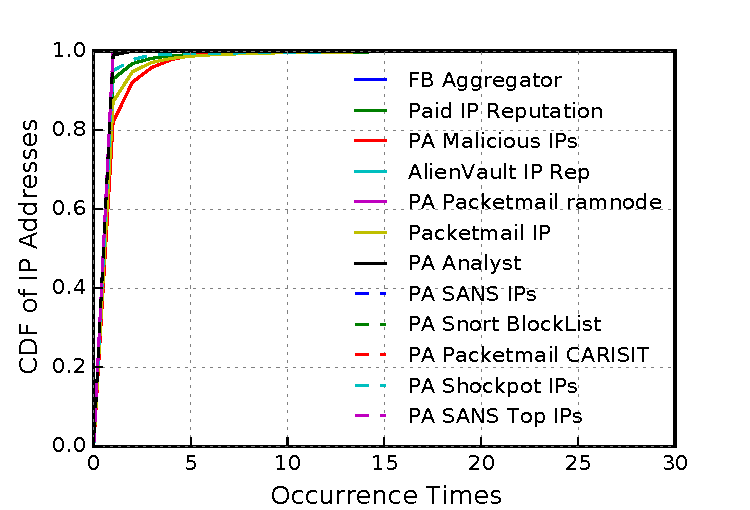
\includegraphics[width=\linewidth]{images/scan_occurrence.pdf}
\caption{CDF of scan feeds data occurrence}
\label{fig:scan_occurrence}
\end{subfigure}\hspace*{\fill}
\begin{subfigure}{0.33\textwidth}
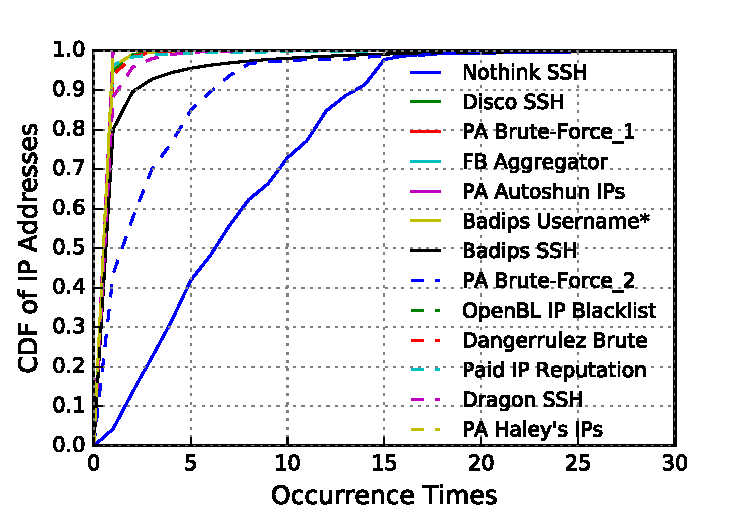
\includegraphics[width=\linewidth]{images/brute_occurrence.pdf}
\caption{CDF of brute-force feeds data occurrence}
\label{fig:brute_occurrence}
\end{subfigure}\hspace*{\fill}
\begin{subfigure}{0.33\textwidth}
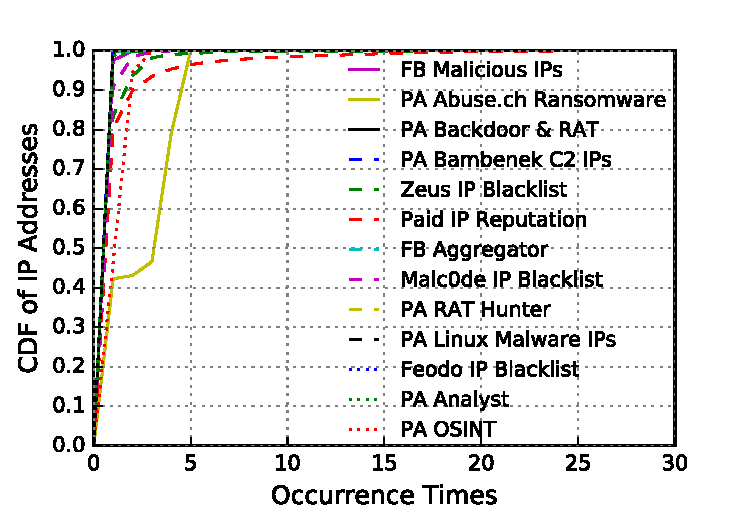
\includegraphics[width=\linewidth]{images/malware_occurrence.pdf}
\caption{CDF of malware feeds data occurrence}
\label{fig:malware_occurrence}
\end{subfigure}
%\medskip

\caption{CDF of data occurrence}
\end{figure*}


Although most data only occurred once, there are some noticeable expectations. For the feed {\feedTSAbusech} in malware category, we have 6 months of its data, however, 32.5\% of its IPs occurred 4 times and 20.9\% of IPs occurred 5 times during this time. We checked the intervals between each occurrence and found over 97\% of the intervals are in the range 30-36 days. This indicates that this feed captured a lot of monthly events. The feed {\feednothink} in graph~\ref{fig:brute_occurrence} shows a bizarre straight line. Diving into the feed's data we found that this feed redistribute all its previous data every 30 days. Similar behavior also showed up in feed {badips-drupal} and {badips-vsftpd}. \note{talk about the result after removing the redistribution}.

The occurrence count of an IP reveals the predictability of this data point over the time. A bad IP won't always be bad\note{need example: scanning IP won't scan forever, botnet host change IPs, c2 server change IPs, citation needed}. If an IP shows up in a feed and never show up again, then the value this data point has is limited to a very short time window. The fact that most data in a feed only show up once means that threat intelligence data are very time sensitive.



%%% ========================================
%%% Volume for proxy and ddos
%%%

\begin{table*}
\small
\caption{Summary of proxy feeds}
\centering
 \begin{tabular}{l l l l l l c c}
 \toprule
 Feed & Duration & IP Count & Daily IPs & /24 Count & /24 over IPs & Format & Attribute\\
 \midrule
 {\feedetiprep}                  & 2015-11 - 2017-12 & 130751 & 165 & 72233 & 0.55 & \snapfeedsym & \aggfeedsym\\
 {TS TOR Exit Nodes}                 & 2015-11 - 2016-08 & 130160 & 464 & 70629 & 0.54 & \deltafeedsym & \singlefeedsym\\
 {TS Anomali Labs TOR Nodes}         & 2015-11 - 2016-08 & 121324 & 407 & 62335 & 0.51 & \deltafeedsym & \singlefeedsym\\
 {FB Facebook Administrator}         & 2015-11 - 2017-06 & 22033 & 37 & 14118 & 0.64 & \deltafeedsym & \aggfeedsym\\
 {TS Labs I2P Relay Nodes*}          & 2015-11 - 2016-07 & 21531 & 88 & 19621 & 0.91 & \deltafeedsym & \singlefeedsym\\
 %TS Anomali Labs I2P Relay Nodes
 {FB Tor Exit Nodes}                 & 2016-06 - 2017-12 & 18231 & 31 & 10339 & 0.56 & \deltafeedsym & \singlefeedsym\\
 {FB PayPal Intel Sharing}           & 2015-11 - 2016-09 & 4839 & 15 & 4261 & 0.88 & \deltafeedsym & \aggfeedsym\\
 {\feedFBZendesk}         & 2015-11 - 2017-06 & 4457 & 7 & 3122 & 0.70 & \deltafeedsym & \aggfeedsym\\
 {TS Maxmind Proxy List}             & 2015-12 - 2016-08 & 3066 & 12 & 2479 & 0.80 & \deltafeedsym & \singlefeedsym\\
 {badips-proxy}                      & 2015-11 - 2017-12 & 2604 & 3 & 2081 & 0.79 & \snapfeedsym & \singlefeedsym\\
\bottomrule
\end{tabular}
\label{tab:proxy-overview}
\end{table*}

\begin{table*}
\small
\caption{Summary of DDoS feeds}
\centering
 \begin{tabular}{l l l l l l c c}
 \toprule
 Feed & Duration & IP Count & Daily IPs & /24 Count & /24 over IPs & Format & Attribute\\
 \midrule
{FB Netflix SIRT}        & 2015-11 - 2017-11 & 157620 & 209 & 112243 & 0.71 & \deltafeedsym & \aggfeedsym\\
{\feedetiprep}       & 2015-11 - 2017-12 & 19136 & 24 & 7845 & 0.40 & \snapfeedsym & \aggfeedsym\\
{badips-apacheddos}      & 2015-11 - 2017-12 & 17560 & 22 & 11604 & 0.66 & \snapfeedsym & \singlefeedsym\\
\bottomrule
\end{tabular}
\label{tab:ddos-overview}
\end{table*}


%%% ============================================
%%% Geo analysis
%%%

% We might not need this geo location analysis since it doesn't offer us too many information.
By analyzing the geographic distributions of IP addresses by category, we can see if there are trends among the categories, as well as test our categorization methodology by seeing if they follow well-known trends for certain categories such as scans. In order to calculate this data, we use MaxMind's publicly available databases for IP Addresses. We analyze this on the country level, although MaxMind also provides city and ASN databases.

The geographic distribution of IP addresses is plotted by category. Only unique IP addresses are counted for these percentages, so that multiple submissions would not skew the distribution of alleged malicious IPs. In the plot, only the top 20 countries by percentage are shown for each category, as the tails of the distribution are quite long. As seen in the plot, each of the different categories presents different patterns in their geographic distributions. However, they also show similarities, with the United States, China, and Russia showing up in similar percentages across most categories. One exception to the general shape of the graph is the proxy category, which shows an almost thirty-five percent distribution coming from Germany IP addresses. Although less dramatic, the malware category shows some skew as well, with almost twenty-five percent coming from Brazil. The entire distribution can be seen below.
\begin{figure}[h]
\label{Table 16: Geographic Location Distribution: Country}
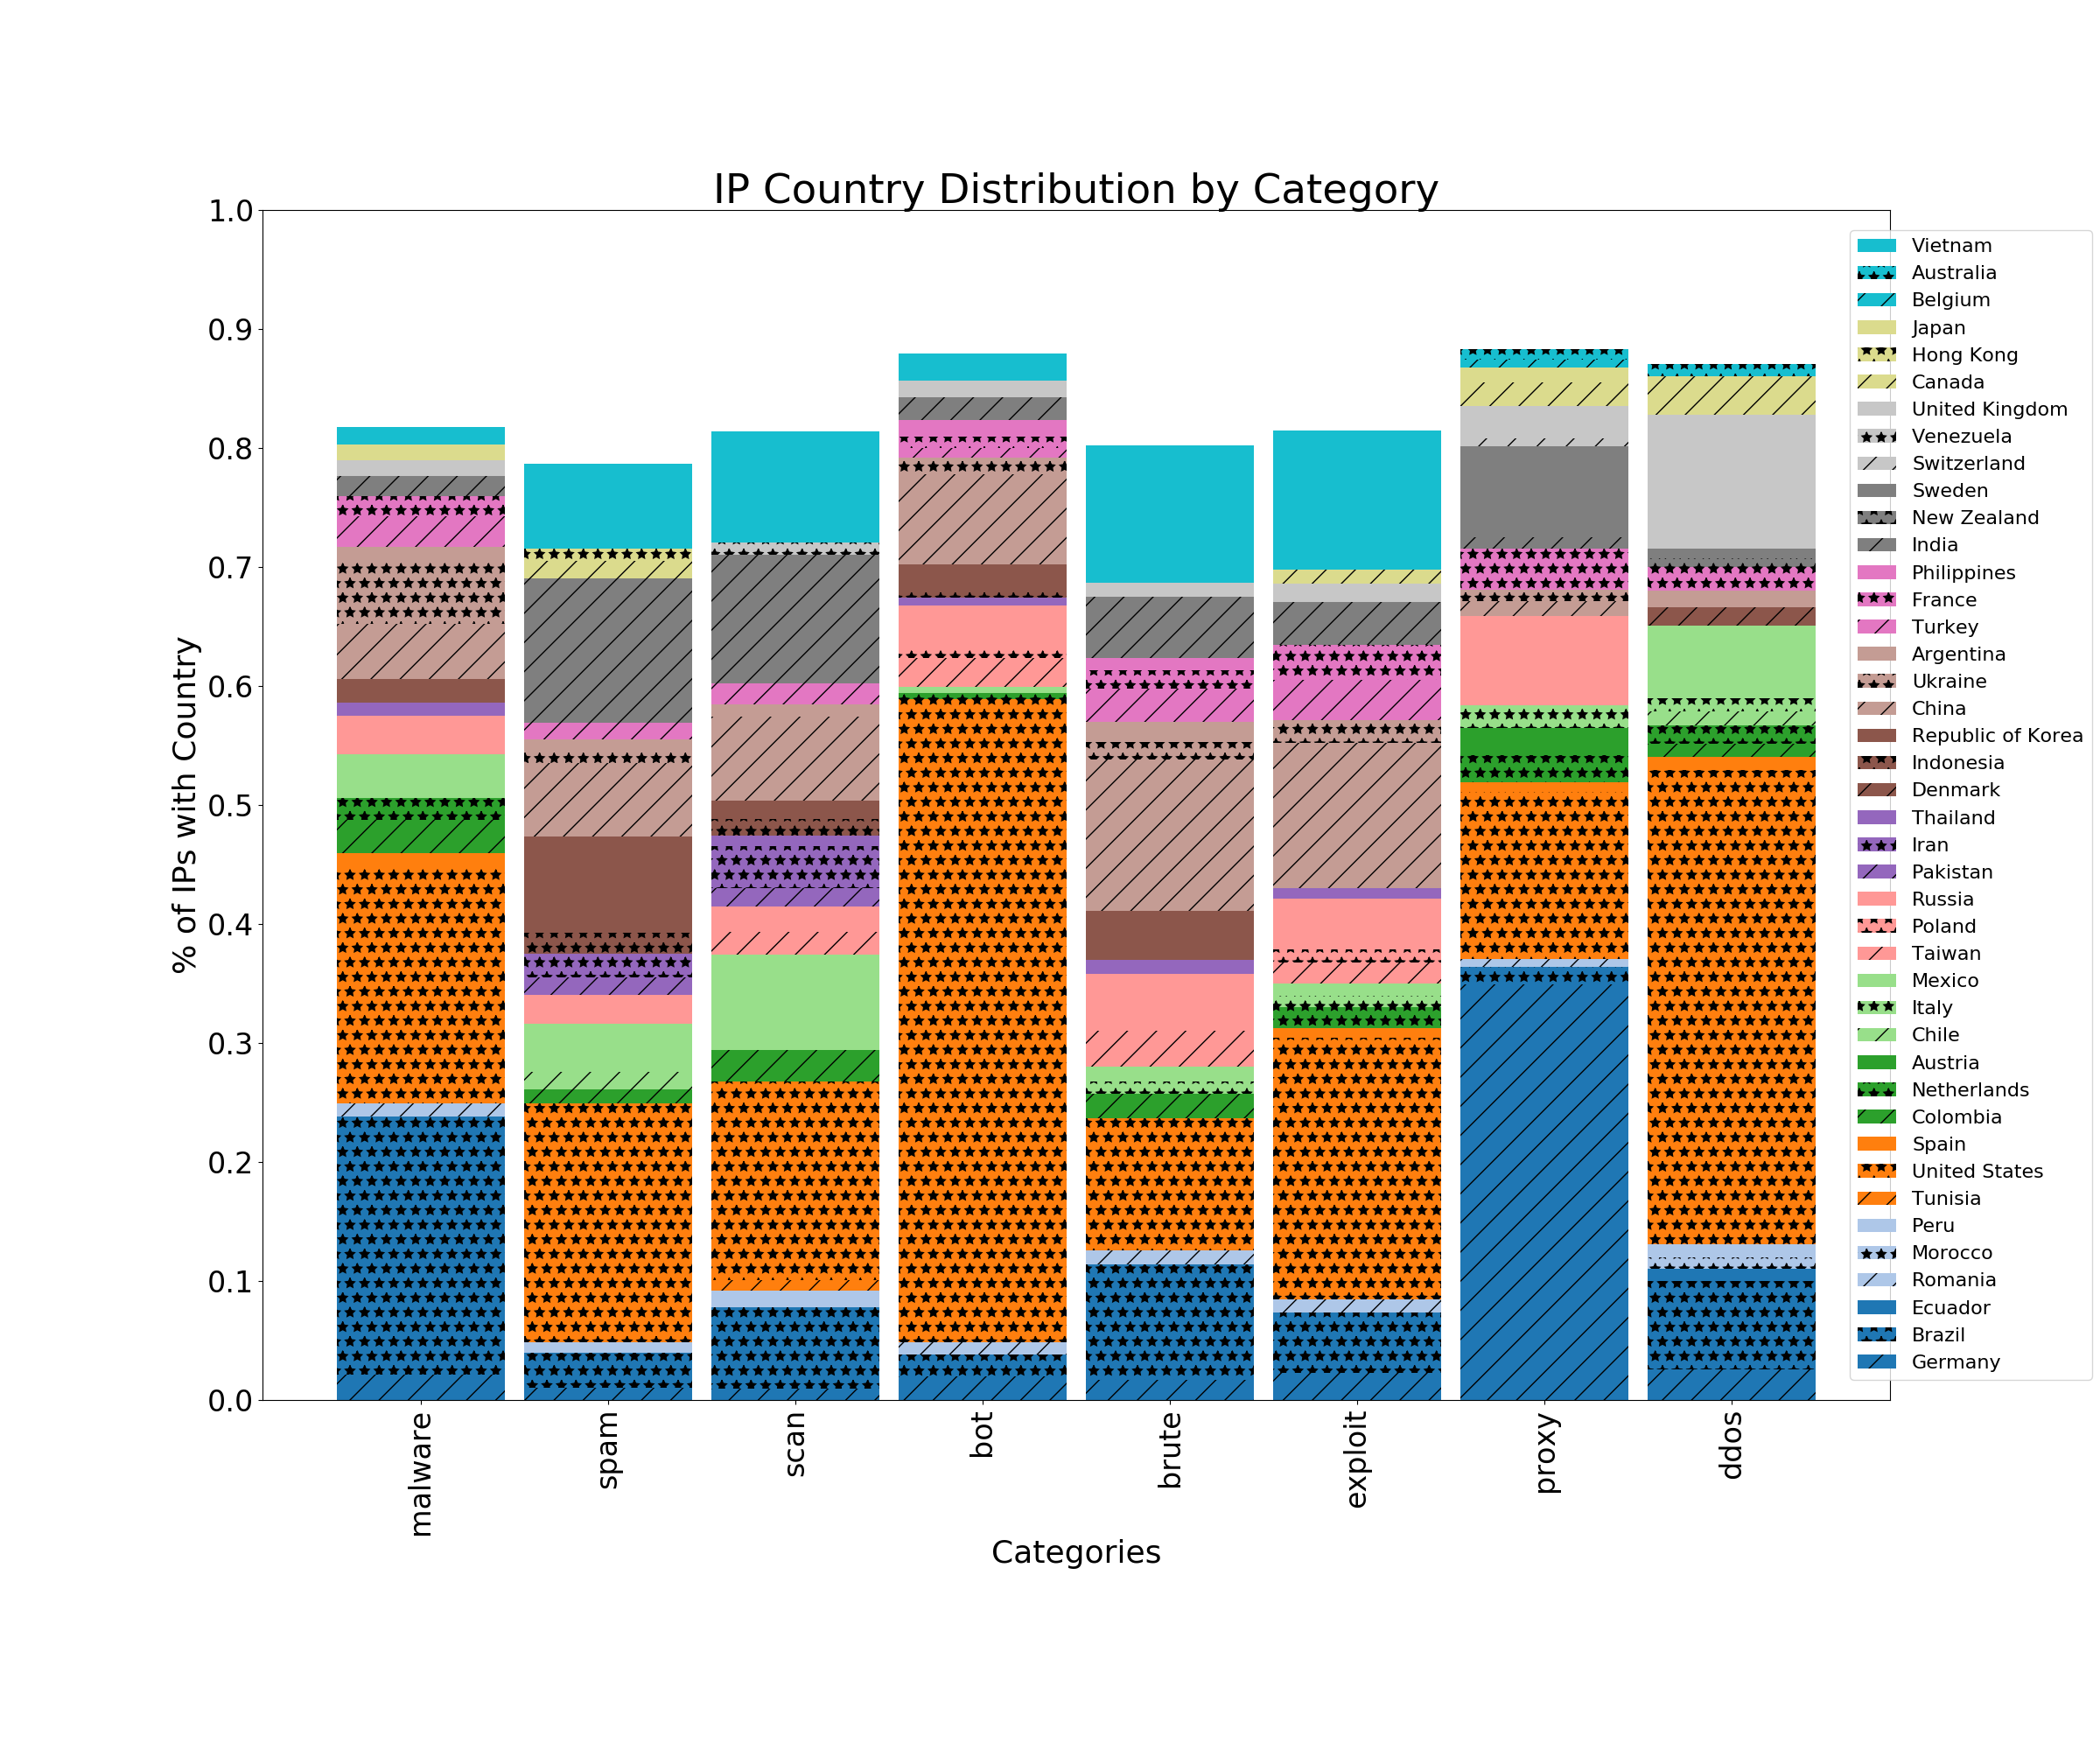
\includegraphics[width=\columnwidth]{images/categoryGeoIP.png}
\caption{Country Distribution by IP Category}
\end{figure}

%%% ===========================================
%%% Unique contribution
%%%
\begin{table}
\footnotesize
\caption{Unique contribution of scan feeds}
\centering
 \begin{tabular}{r l l l}
 \toprule
 Feed & IP Count & Unique IPs & Rate \\
 \midrule
 \multirow{1}{*}{{\feedetiprep}}                 & 506840 & 498220 & 98.2\% \\%& 3343627 & 3253440 & 97.3\% \\
 \multirow{1}{*}{{TS Snort IP BlockList}}        & 361072 & 360063 & 99.7\% \\ %& 361072 & 357511 & 99.0\% \\
 \multirow{1}{*}{{\feedpacketmail}}                & 79866 & 70663 & 88.4\% \\ %& 637732 & 555757 & 87.1\% \\
 \multirow{1}{*}{{TS Packetmail$_1$}}            & 17366 & 13899 & 80.0\% \\ %& 17366 & 12984 & 74.7\% \\
 \multirow{1}{*}{{TS Labs MHN Community*}}       & 11275 & 6512 & 57.7\% \\ %& 11275 & 6008 & 53.2\% \\
 \multirow{1}{*}{{\feedalienvault}}              & 9087 & 6374 & 70.1\% \\ %& 41395 & 23544 & 56.8\% \\
 \multirow{1}{*}{{TS Packetmail$_2$}}            & 3228 & 1533 & 47.4\% \\ %& 3228 & 1419 & 43.9\% \\
 \multirow{1}{*}{{FB Basecamp Streetcred}}       & 3162 & 2817 & 89.0\% \\ %& 3772 & 3210 & 85.1\% \\
 \multirow{1}{*}{{TS SANS Top IPs}}              & 2865 & 1655 & 57.7\% \\ %& 2865 & 1520 & 53.0\% \\
\bottomrule
\end{tabular}
\label{tab:scan-unique}
\end{table}


\begin{table}
\footnotesize
\caption{Unique contribution of brute-force feeds}
\centering
 \begin{tabular}{r l l l}
 \toprule
 Feed & IP Count & Unique IPs & Rate \\
 \midrule
\multirow{1}{*}{{\feedbadipssh}}                    & 446346 & 86528 & 19.3\% \\ %& 4857417 & 931135 & 19.1\% \\
\multirow{1}{*}{{badips-telnet}}                 & 331845 & 10 & 0.00\% \\ %& 3553580 & 539 & 0.01\% \\
\multirow{1}{*}{{\feedetiprep}}                  & 223903 & 201849 & 90.1\% \\ %& 2423436 & 2048567 & 84.5\% \\
\multirow{1}{*}{{TS Blocklist Brute Force}}      & 187789 & 181905 & 96.8\% \\ %& 187789 & 175192 & 93.2\% \\
\multirow{1}{*}{{\feedopenbl}}         & 15571 & 4287 & 27.5\% \\ %& 48624 & 10527 & 21.6\% \\
\multirow{1}{*}{{\feeddragon}}                    & 10909 & 3853 & 35.3\% \\ %& 10909 & 3635 & 33.3\% \\
\multirow{1}{*}{{\feeddangerrule}}             & 10339 & 872 & 8.43\% \\ %& 33977 & 2064 & 6.07\% \\
\multirow{1}{*}{{TS Autoshun w/o tags}}          & 4959 & 1943 & 39.1\% \\ %& 4959 & 1839 & 37.0\% \\
\multirow{1}{*}{{FB Zendesk ThreatExchange}}     & 4470 & 1871 & 41.8\% \\ %& 37885 & 8797 & 23.2\% \\
\multirow{1}{*}{{\feednothink}}                   & 3191 & 1682 & 52.7\% \\ %& 12713 & 5519 & 43.4\% \\
\multirow{1}{*}{{\feeddisco}}                     & 2174 & 314 & 14.4\% \\ %& 22693 & 4252 & 18.7\% \\
\multirow{1}{*}{{badips-username-notfound}}      & 1760 & 310 & 17.6\% \\ %& 25939 & 12114 & 46.7\% \\
\bottomrule
\end{tabular}
\label{tab:brute-unique}
\end{table}


\begin{table}
\footnotesize
\caption{Unique contribution of malware feeds}
\centering
 \begin{tabular}{r l l l}
 \toprule
 Feed & IP Count & Unique IPs & Rate \\
 \midrule
\multirow{1}{*}{{\feedetiprep}}                  & 204582 & 192869 & 94.2\% \\%& 538414 & 524689 & 97.4\% \\
\multirow{1}{*}{{FB Facebook Administrator}}     & 110713 & 110456 & 99.7\% \\%& 148096 & 147527 & 99.6\% \\
\multirow{1}{*}{{TS Virbl - DNS Blacklist}}      & 17309 & 17273 & 99.7\% \\%& 17309 & 17263 & 99.7\% \\
\multirow{1}{*}{{TS Alien Vault - Malware}}      & 14040 & 13550 & 96.5\% \\%& 14040 & 13453 & 95.8\% \\
\multirow{1}{*}{{TS Abuse.ch Ransomware IPs}}    & 10673 & 250 & 2.34\% \\%& 10673 & 14 & 0.13\% \\
\multirow{1}{*}{{FB Zendesk ThreatExchange}}     & 1964 & 1884 & 95.9\% \\%& 3083 & 2827 & 91.6\% \\
\multirow{1}{*}{{TS Anomali Labs RAT Hunter}}    & 3413 & 2939 & 86.1\% \\%& 3413 & 2800 & 82.0\% \\
\multirow{1}{*}{{\feedmalcode}}        & 619 & 355 & 57.3\% \\%& 2721 & 1512 & 55.5\% \\
\multirow{1}{*}{{TS Analyst}}                    & 1853 & 1312 & 70.8\% \\%& 1853 & 1196 & 64.5\% \\
\bottomrule
\end{tabular}
\label{tab:malware-unique}
\end{table}



\begin{table}
\footnotesize
\caption{Unique contribution of botnet feeds}
\centering
 \begin{tabular}{r l l l}
 \toprule
 Feed & IP Count & Unique IPs & Rate \\
 \midrule
\multirow{1}{*}{{\feedetiprep}}                  & 213740 & 211430 & 98.9\% \\ %& 422542 & 420007 & 99.4\% \\
\multirow{1}{*}{{TS Anomali Labs MHN}}           & 147904 & 111750 & 75.5\% \\ %& 147904 & 111640 & 75.4\% \\
\multirow{1}{*}{{TS Anomali Labs MHN Tagged}}    & 34727 & 4644 & 13.3\% \\ %& 34727 & 4641 & 13.3\% \\
\multirow{1}{*}{{TS Blocklist Bots}}             & 32065 & 26145 & 81.5\% \\ %& 32065 & 26125 & 81.4\% \\
\multirow{1}{*}{{TS Botscout BOT IPs}}           & 22578 & 16809 & 74.4\% \\ %& 22578 & 16800 & 74.4\% \\
\multirow{1}{*}{{TS CI Army}}                    & 18087 & 13233 & 73.1\% \\ %& 18087 & 13213 & 73.0\% \\
\multirow{1}{*}{{TS ET - Compromised}}           & 5853 & 2937 & 50.1\% \\ %& 5853 & 2935 & 50.1\% \\
\multirow{1}{*}{{FB Zendesk ThreatExchange}}     & 2898 & 2811 & 96.9\% \\ %& 3292 & 3199 & 97.1\% \\
\multirow{1}{*}{{TS VoIP Blacklist}}             & 2825 & 2135 & 75.5\% \\ %& 2825 & 2133 & 75.5\% \\
\bottomrule
\end{tabular}
\label{tab:bot-unique}
\end{table}


\begin{table}
\footnotesize
\caption{Unique contribution of exploit feeds}
\centering
 \begin{tabular}{r l l l}
 \toprule
 Feed & IP Count & Unique IPs & Rate \\
 \midrule
\multirow{1}{*}{{\feedbadiphttp}}               & 341527 & 85740 & 25.1\% \\
\multirow{1}{*}{{badips-cms}}                & 199842 & 9 & 0.00\% \\
\multirow{1}{*}{{\feedbadipftp}}                & 168160 & 99946 & 59.4\% \\
\multirow{1}{*}{{badips-wordpress}}          & 119619 & 1 & 0.00\% \\
\multirow{1}{*}{{badips-apache}}             & 59398 & 4 & 0.00\% \\
\multirow{1}{*}{{badips-proftpd}}            & 42142 & 3 & 0.00\% \\
\multirow{1}{*}{{badips-pureftpd}}           & 39105 & 5 & 0.01\% \\
\multirow{1}{*}{{\feedbadipdns}}                & 35119 & 34889 & 99.3\% \\
\multirow{1}{*}{{badips-vsftpd}}             & 8944 & 1 & 0.01\% \\
\multirow{1}{*}{{FB Zendesk ThreatExchange}} & 5615 & 4507 & 80.2\% \\
\multirow{1}{*}{{badips-drupal}}             & 6180 & 0 & 0.0\% \\
\multirow{1}{*}{{badips-wp}}                 & 6503 & 0 & 0.0\% \\
\multirow{1}{*}{{badips-apache-scriddies}}   & 3482 & 0 & 0.0\% \\
\multirow{1}{*}{{\feedbadiprfi}}         & 3200 & 2210 & 69.0\% \\
\multirow{1}{*}{{\feedbadipxml}}             & 2190 & 1310 & 59.8\% \\
\bottomrule
\end{tabular}
\label{tab:exploit-unique}
\end{table}


\begin{table}
\footnotesize
\caption{Unique contribution of spam feeds}
\centering
 \begin{tabular}{r l l l}
 \toprule
 Feed & IP Count & Unique IPs & Rate \\
 \midrule
\multirow{1}{*}{{\feedbadippostfix}}                & 421797 & 404697 & 95.9\% \\ %& 2007178 & 1860760 & 92.7\% \\
\multirow{1}{*}{{\feedetiprep}}                  & 287859 & 286435 & 99.5\% \\ %& 1195954 & 1187074 & 99.2\% \\
\multirow{1}{*}{{\feedbadipspam}}                   & 2742 & 990 & 36.1\% \\ %& 254047 & 138033 & 54.3\% \\
\multirow{1}{*}{{FB Zendesk ThreatExchange}}     & 40869 & 27051 & 66.1\% \\ %& 79653 & 40905 & 51.3\% \\
\multirow{1}{*}{{TS Spamhaus}}                   & 49712 & 47868 & 96.2\% \\ %& 49712 & 42583 & 85.6\% \\
\multirow{1}{*}{{\feedalienvault}}               & 10098 & 8649 & 85.6\% \\ %& 32598 & 28915 & 88.7\% \\
\multirow{1}{*}{{TS Bot Scout IP}}               & 10018 & 9571 & 95.5\% \\ %& 10018 & 9377 & 93.6\% \\
\multirow{1}{*}{{TS Spamhaus Extended}}          & 9526 & 8710 & 91.4\% \\ %& 9526 & 8665 & 90.9\% \\
\bottomrule
\end{tabular}
\label{tab:spam-unique}
\end{table}
